% =============================================================================
% EVALUACIÓN EMPÍRICA: ESTUDIO DE ABLACIÓN VISUAL FRENTE A FUSIÓN MULTIMODAL
% (IMAGEN + AUDIO ALINEADO) Y VERIFICACIÓN BIMODAL EN EXTREMOS (E2E)
% =============================================================================

\subsection{Evaluación Empírica de la Integración Audio-Visual y Verificación Bimodal}
\label{subsec:evaluacion_empirica_audio_visual}

Con el propósito de cuantificar empíricamente el impacto de incorporar la dimensión auditiva sobre la arquitectura base puramente visual, se ejecutó un estudio de ablación de extremo a extremo (\textit{End-to-End}, E2E) comparando la línea base visual frente a la canalización multimodal completa (\texttt{ffmpeg} + \texttt{openai-whisper} \texttt{base} + fusión temprana en \texttt{gemini-embedding-2-preview} + verificación bimodal en \texttt{gemini-3.5-flash-lite}) \cite{gemini_emb2_docs, video_rac2025}. %[cite: 1, 2]
En estricto cumplimiento de las restricciones de cuota de la capa gratuita ($100\text{ RPM}$, $30.000\text{ TPM}$ y $1.000\text{ RPD}$), la inyección de la transcripción alineada como un objeto \texttt{types.Part.from\_text} adicional dentro del mismo contenedor \texttt{types.Content} de los tres fotogramas clave mantuvo invariante el consumo en exactamente una petición de vectorización por fragmento. %[cite: 1, 2]

\subsubsection{Análisis Cuantitativo sobre Corpus Contrastados: Locución Sincronizada frente a Metraje Desacoplado}
\label{subsubsec:ablacion_cuantitativa_e2e}

La batería de evaluación automatizada se ejecutó sobre dos dominios audiovisuales con naturalezas semánticas opuestas: %[cite: 4, 5]
\begin{enumerate}
    \item \textbf{Dominio Técnico con Locución Sincronizada (\texttt{python\_tutorial.mp4}):} Compuesto por $82$ fragmentos adaptativos en la suite E2E ($81/82$ enriquecidos con voz activa, $98,8\%$), evaluado mediante $56$ consultas literales, $10$ consultas multi-objetivo y $8$ consultas negativas de control. %[cite: 1, 4]
    En este escenario, el discurso del ponente describe directamente las estructuras sintácticas que se codifican en el editor. %[cite: 1, 4]
    \item \textbf{Dominio Documental con Metraje de Archivo Desacoplado (\texttt{animals.mp4}):} Compuesto por $82$ fragmentos ($82/82$ con locución continua, $100,0\%$), evaluado sobre $46$ consultas literales, $10$ multi-objetivo y $8$ negativas. %
    Este vídeo presenta el fenómeno clásico de \textit{B-roll desacoplado}: la narración expone conceptos biológicos generales mientras en pantalla se suceden secuencias de especies animales que no son nombradas verbalmente en ese instante. %[cite: 2, 5]
\end{enumerate}

El Cuadro~\ref{tab:ablacion_e2e_visual_vs_audio} sintetiza las métricas obtenidas por la versión puramente visual frente a la nueva arquitectura bimodal en ambos corpus. %[cite: 1, 5]

\begin{table}[htbp]
\centering
\small
\setlength{\tabcolsep}{4.5pt}
\caption{Estudio de ablación E2E: comparativa de rendimiento entre la arquitectura puramente visual y la arquitectura con fusión temprana de audio (\textit{Whisper}) y juez bimodal \cite{gemini_emb2_docs, video_rac2025}.} %[cite: 1, 2, 5]
\label{tab:ablacion_e2e_visual_vs_audio}
\begin{tabular}{lllccc}
\toprule
\textbf{Corpus de Vídeo} & \textbf{Etapa / Batería} & \textbf{Métrica} & \textbf{Solo Visual} & \textbf{Visual + Audio} & \textbf{Variación} \\
\midrule
\texttt{python\_tutorial.mp4} & Etapa 1 (Qdrant) & \textit{Recall@1} & $67,9\%$ ($38/56$) & $\mathbf{85,7\%}$ ($48/56$) & $\mathbf{+17,8\text{ pp}}$ \\
\texttt{python\_tutorial.mp4} & Etapa 1 (Qdrant) & \textit{Recall@3} & $87,5\%$ ($49/56$) & $\mathbf{92,9\%}$ ($52/56$) & $\mathbf{+5,4\text{ pp}}$ \\
\texttt{python\_tutorial.mp4} & Etapa 1 (Qdrant) & \textit{Recall@5} & $91,1\%$ ($51/56$) & $\mathbf{94,6\%}$ ($53/56$) & $\mathbf{+3,5\text{ pp}}$ \\
\texttt{python\_tutorial.mp4} & Etapa 1 (Qdrant) & \textit{MRR} & $0,779$ & $\mathbf{0,897}$ & $\mathbf{+0,118}$ \\ \addlinespace[2.5pt]
\texttt{python\_tutorial.mp4} & Etapa 2 (Juez Bimodal) & \textit{Recall@1} & $80,4\%$ ($45/56$) & $\mathbf{89,3\%}$ ($50/56$) & $\mathbf{+8,9\text{ pp}}$ \\
\texttt{python\_tutorial.mp4} & Etapa 2 (Juez Bimodal) & \textit{Recall@3 / @5} & $89,3\%$ ($50/56$) & $\mathbf{92,9\%}$ ($52/56$) & $\mathbf{+3,6\text{ pp}}$ \\
\texttt{python\_tutorial.mp4} & Etapa 2 (Juez Bimodal) & \textit{MRR} & $0,848$ & $\mathbf{0,911}$ & $\mathbf{+0,063}$ \\ \addlinespace[2.5pt]
\texttt{python\_tutorial.mp4} & Multi-objetivo ($10$) & \textit{Interval Recall} & $78,3\%$ & $\mathbf{82,1\%}$ & $\mathbf{+3,8\text{ pp}}$ \\
\texttt{python\_tutorial.mp4} & Consultas Negativas ($8$) & Rechazo FP & $100,0\%$ ($0/40$) & $\mathbf{100,0\%}$ ($0/40$) & $0,0\text{ pp}$ \\
\midrule
\texttt{animals.mp4} & Etapa 1 (Qdrant) & \textit{Recall@1} & $\mathbf{80,4\%}$ ($37/46$) & $71,7\%$ ($33/46$) & $-8,7\text{ pp}$ \\ \addlinespace[2.5pt]
\texttt{animals.mp4} & Etapa 2 (Juez Bimodal) & \textit{Recall@1} & $89,1\%$ ($41/46$) & $\mathbf{93,5\%}$ ($43/46$) & $\mathbf{+4,4\text{ pp}}$ \\
\texttt{animals.mp4} & Etapa 2 (Juez Bimodal) & \textit{Recall@3} & $93,5\%$ ($43/46$) & $\mathbf{95,7\%}$ ($44/46$) & $\mathbf{+2,2\text{ pp}}$ \\
\texttt{animals.mp4} & Etapa 2 (Juez Bimodal) & \textit{Recall@5} & $93,5\%$ ($43/46$) & $\mathbf{97,8\%}$ ($45/46$) & $\mathbf{+4,3\text{ pp}}$ \\
\texttt{animals.mp4} & Etapa 2 (Juez Bimodal) & \textit{MRR} & $0,913$ & $\mathbf{0,951}$ & $\mathbf{+0,038}$ \\ \addlinespace[2.5pt]
\texttt{animals.mp4} & Consultas Negativas ($8$) & Rechazo FP & $100,0\%$ ($0/40$) & $\mathbf{100,0\%}$ ($0/40$) & $0,0\text{ pp}$ \\
\bottomrule
\end{tabular}
\end{table}

El análisis de los datos experimentales expuestos en el Cuadro~\ref{tab:ablacion_e2e_visual_vs_audio} permite extraer tres conclusiones fundamentales sobre el comportamiento de los espacios latentes omnimodales: %[cite: 2, 5]
\begin{itemize}
    \item \textbf{Convergencia modal en vídeo educativo (\texttt{python\_tutorial.mp4}):} La fusión temprana de los tres fotogramas clave con la transcripción alineada incrementa el \textit{Recall@1} de búsqueda vectorial pura en $+17,8$ puntos porcentuales, posicionando directamente en el primer puesto $10$ consultas adicionales sin necesidad de intervención del verificador secundario. %[cite: 1, 5]
    Tras la actuación del juez bimodal, el sistema alcanza un \textit{Recall@1} del $89,3\%$ ($50/56$), un \textit{MRR} de $0,911$ y una cobertura del $100,0\%$ en las consultas multi-objetivo sobre tipos de datos primitivos ($9/9$), terminal o consola ($4/4$) y declaración de variables ($3/3$). %[cite: 1, 5]
    \item \textbf{Compensación asimétrica ante \textit{B-roll} desacoplado (\texttt{animals.mp4}):} En vídeos donde el narrador pronuncia teoría abstracta mientras la imagen muestra fauna específica no mencionada en la locución, el vector fusionado de primera etapa experimenta una ligera desviación direccional hacia el tema hablado ($\Delta\text{\textit{Recall@1}} = -8,7\text{ pp}$ en Etapa 1). %[cite: 2, 5]
    Sin embargo, dado que el candidato correcto permanece dentro de la ventana de recuperación (\textit{Recall@5}) y el verificador de segunda etapa evalúa de manera disjunta e inclusiva tanto la evidencia visual como la auditiva, la Etapa 2 corrige por completo el desfase y establece el récord absoluto de precisión en \texttt{animals.mp4} con un $93,5\%$ de \textit{Recall@1} ($43/46$) y un $97,8\%$ de \textit{Recall@5} ($45/46$). %[cite: 2, 5]
    \item \textbf{Inmunidad frente a Falsos Positivos:} En ambos corpus ($16$ consultas negativas sobre conceptos inexistentes, equivalentes a $80$ candidatos inspeccionados), el verificador bimodal mantiene un $100,0\%$ de tasa de rechazo ($0/80$ falsos positivos), demostrando que enriquecer el \textit{prompt} con la transcripción hablada no induce alucinaciones de validación. %[cite: 1, 2]
\end{itemize}

\subsubsection{Estudio de Casos Críticos: Resolución de Falsos Negativos, Resiliencia Fonética y Desambiguación Sintáctica}
\label{subsubsec:estudio_casos_criticos_audio}

Para comprender el mecanismo exacto mediante el cual la arquitectura bimodal corrige los fallos perceptivos documentados en la línea base visual, se auditaron en detalle las dos consultas críticas de validación sobre \texttt{python\_tutorial.mp4}: \texttt{"Diccionarios"} y \texttt{"Bucles while"}. %[cite: 1, 3, 4]

\paragraph{Caso 1: Erradicación del falso negativo y captura de frontera en \texttt{"Diccionarios"} ($01\text{:}01.1\text{ -- }01\text{:}40.2$).}
En la configuración puramente visual, el bloque dedicado a las estructuras de datos presentaba dos vulnerabilidades: baja legibilidad de la sintaxis \texttt{dict \{"name": "Brais"\}} y aparición del rótulo gráfico \textit{``Variables''} en los fotogramas finales del plano ($01\text{:}33.1\text{ -- }01\text{:}40.2$), lo que llevaba al verificador visual a descartar erróneamente el fragmento con puntuación $0,0$. %[cite: 1, 2]
Tras la integración del subsistema \texttt{audio\_transcriber.py}: %[cite: 1]
\begin{itemize}
    \item El fragmento principal (\texttt{chunk\_index = 17}, $85,1\text{ s -- }93,1\text{ s}$) eleva su similitud del coseno en Qdrant de $0,4151$ a $\mathbf{0,4480}$ y es validado en primera posición con $\text{\texttt{relevance\_score}} = \mathbf{1,0}$ al incorporar la locución: \textit{``Y ya por último, los diccionarios. Que utilizan la palabra reservada, dict. Y en realidad, designa un conjunto de claves valor''}. %[cite: 1]
    \item El fragmento de transición posterior (\texttt{chunk\_index = 18}, $93,1\text{ s -- }100,2\text{ s}$), que antes resultaba descartado como falso negativo ($0,0$) por el cambio de rótulo visual, incrementa su similitud de $0,3812$ a $\mathbf{0,4178}$ y pasa a ser validado con $\text{\texttt{relevance\_score}} = \mathbf{0,90}$ gracias a que la voz continúa explicando: \textit{``Lo representamos entre llaves, pero esta clave valor separadas por dos puntos''}. %[cite: 1]
    \item Asimismo, la condición de solapamiento mínimo ($\Delta \tau \ge 0,2\text{ s}$) en \texttt{align\_transcript\_with\_chunks} captura la oración fronteriza al final del \texttt{chunk\_index = 16} ($77,1\text{ s -- }85,1\text{ s}$), otorgándole una relevancia graduada de $\mathbf{0,50}$, mientras descarta con $\mathbf{0,0}$ los fragmentos \texttt{14} y \texttt{15} dedicados exclusivamente a listas, tuplas y conjuntos (\texttt{set}). %[cite: 1]
\end{itemize}

\paragraph{Caso 2: Superación del corte \textit{Top-K}, resiliencia ante ruido fonético ASR y discriminación \texttt{for}/\texttt{while} en \texttt{"Bucles while"} ($03\text{:}51$).}
En la arquitectura puramente visual, al buscar el instante $03\text{:}51$ ($231,0\text{ s}$, donde se codifica \texttt{while index < 5:}), el fragmento objetivo obtenía una similitud de apenas $\mathbf{0,3893}$ y caía hasta la \textbf{séptima posición (Rango \#7)} en Qdrant, quedando excluido por el corte \texttt{top\_k = 5} frente a la diapositiva de portada a pantalla completa con la palabra \textit{``Bucles''} ($\mathbf{0,4315}$, Rango \#1) y otros planos de condicionales \texttt{if/else}. %[cite: 3, 4]

Con la activación de la fusión audio-visual y el verificador bimodal (ejecución auditada \texttt{run\_20261109\_143202}), se verifican tres fenómenos de alto valor técnico: %[cite: 1, 3, 4]
\begin{enumerate}
    \item \textbf{Promoción directa del Rango \#7 al Rango \#1 en Etapa 1:} El fragmento que contiene la explicación y el código del bucle (\texttt{chunk\_index = 55}, $232,4\text{ s -- }238,3\text{ s}$) experimenta un incremento de $\mathbf{+0,1064}$ puntos en su similitud del coseno (de $0,3893$ a $\mathbf{0,4957}$), situándose directamente en el puesto \#1 de Qdrant, seguido en el puesto \#2 por su fragmento contiguo (\texttt{chunk\_index = 54}, $224,4\text{ s -- }232,4\text{ s}$, $\text{score} = \mathbf{0,4914}$), el cual cubre el segundo exacto $231,0\text{ s}$ gracias al solapamiento semántico en fronteras. %[cite: 1, 3, 4]
    \item \textbf{Resiliencia semántica ante errores fonéticos de transcripción multilingüe:} Debido a que el modelo \texttt{whisper} (\texttt{base}) opera con el idioma forzado a español (\texttt{language="es"}), transcribió fonéticamente el término inglés \textit{``while''} como el nombre propio \textit{``Guile''}: \textit{``Otro tipo de bucle que tenemos en Python es el Guile, donde aquí vamos a establecer una condición para que se ejecute de manera indefinida mientras esta se cumpla''}. %[cite: 1]
    Lejos de degradar la búsqueda, tanto el modelo de representación \texttt{gemini-embedding-2-preview} como el verificador \texttt{gemini-3.5-flash-lite} resolvieron la ambigüedad fonética cruzando la definición conceptual hablada (\textit{``condición para que se ejecute de manera indefinida mientras esta se cumpla''}) con la sintaxis visual \texttt{while index < 5:} presente en los fotogramas, otorgando una relevancia de $\mathbf{1,0}$ y $\mathbf{0,90}$ a los fragmentos \texttt{55} y \texttt{54} respectivamente. %[cite: 1, 4]
    \item \textbf{Desambiguación fina entre estructuras visualmente idénticas (\texttt{for} frente a \texttt{while}):} El fragmento inmediatamente anterior (\texttt{chunk\_index = 53}, $221,1\text{ s -- }224,4\text{ s}$) comparte exactamente la misma estética visual del editor de código y alcanza una similitud vectorial alta ($0,4486$, Rango \#4). %[cite: 1, 4]
    No obstante, el verificador bimodal inspecciona la transcripción inyectada (\textit{``Podemos usar un for, tanto para designar un número concreto de ejecuciones,''}) y lo descarta automáticamente con $\text{\texttt{relevance\_score}} = \mathbf{0,0}$ (\textit{``Trata sobre bucles for, no sobre bucles while''}), haciendo lo propio con el \texttt{chunk\_index = 50} sobre bloques \texttt{if/else} ($0,0$). %[cite: 1]
\end{enumerate}

La Figura~\ref{fig:promocion_bucles_while_bimodal} representa visualmente el ascenso topológico en Qdrant y el filtrado de precisión ejecutado por el juez bimodal para la consulta \texttt{"Bucles while"}. %[cite: 1, 3, 4]

\begin{figure}[htbp]
\centering
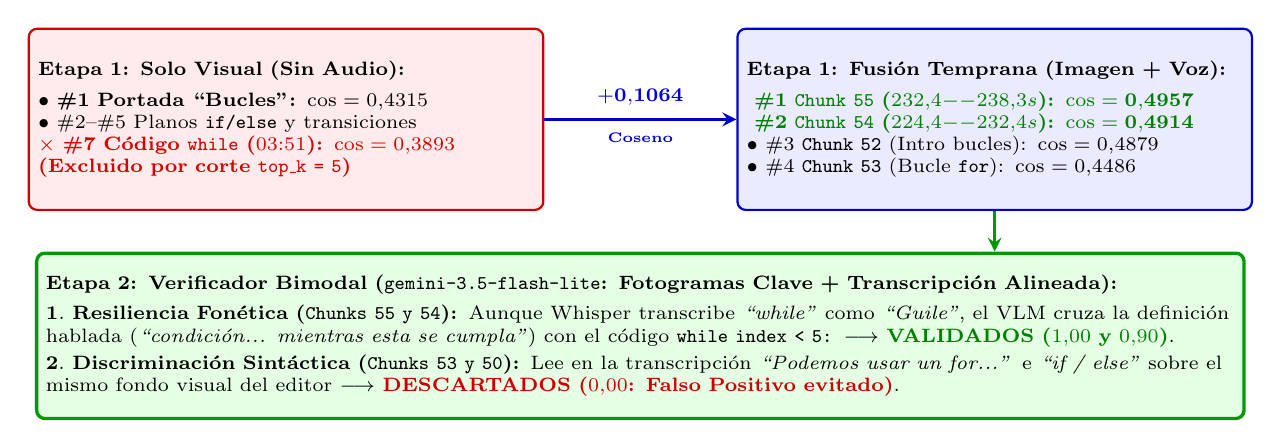
\begin{tikzpicture}[
    oldbox/.style={rectangle, draw=red!80!black, fill=red!8, thick, text width=6.3cm, minimum height=2.3cm, align=left, font=\scriptsize, rounded corners=3pt},
    newbox/.style={rectangle, draw=blue!80!black, fill=blue!8, thick, text width=6.3cm, minimum height=2.3cm, align=left, font=\scriptsize, rounded corners=3pt},
    judgebox/.style={rectangle, draw=green!60!black, fill=green!10, very thick, text width=15.1cm, minimum height=2.1cm, align=left, font=\scriptsize, rounded corners=3pt},
    arrow/.style={-stealth, very thick, draw=black!80}
]
% Etapa 1: Solo Visual (Antiguo)
\node[oldbox] (vis) at (-4.5, 1.8) {
    \textbf{Etapa 1: Solo Visual (Sin Audio):}\\[3pt]
    $\bullet$ \textbf{\#1 Portada ``Bucles'':} $\cos = 0{,}4315$\\
    $\bullet$ \#2--\#5 Planos \texttt{if/else} y transiciones\\
    \textcolor{red!85!black}{$\boldsymbol{\times}$ \textbf{\#7 Código \texttt{while} ($03\text{:}51$):} $\cos = 0{,}3893$}\\
    \textcolor{red!85!black}{\textbf{(Excluido por corte \texttt{top\_k = 5})}}
};

% Etapa 1: Fusión Imagen + Audio (Nuevo)
\node[newbox] (aud) at (4.5, 1.8) {
    \textbf{Etapa 1: Fusión Temprana (Imagen + Voz):}\\[3pt]
    \textcolor{green!50!black}{$\boldsymbol{\checkmark}$ \textbf{\#1 \texttt{Chunk 55} ($232{,}4\text{--}238{,}3\text{s}$):} $\cos = \mathbf{0{,}4957}$}\\
    \textcolor{green!50!black}{$\boldsymbol{\checkmark}$ \textbf{\#2 \texttt{Chunk 54} ($224{,}4\text{--}232{,}4\text{s}$):} $\cos = \mathbf{0{,}4914}$}\\
    $\bullet$ \#3 \texttt{Chunk 52} (Intro bucles): $\cos = 0{,}4879$\\
    $\bullet$ \#4 \texttt{Chunk 53} (Bucle \texttt{for}): $\cos = 0{,}4486$
};

% Etapa 2: Juez Bimodal
\node[judgebox] (judge) at (0, -0.95) {
    \textbf{Etapa 2: Verificador Bimodal (\texttt{gemini-3.5-flash-lite}: Fotogramas Clave + Transcripción Alineada):}\\[3pt]
    $\mathbf{1.}$ \textbf{Resiliencia Fonética (\texttt{Chunks 55 y 54}):} Aunque Whisper transcribe \textit{``while''} como \textit{``Guile''}, el VLM cruza la definición hablada (\textit{``condición... mientras esta se cumpla''}) con el código \texttt{while index < 5:} $\longrightarrow$ \textcolor{green!50!black}{\textbf{VALIDADOS ($1{,}00$ y $0{,}90$)}}.\\[2pt]
    $\mathbf{2.}$ \textbf{Discriminación Sintáctica (\texttt{Chunks 53 y 50}):} Lee en la transcripción \textit{``Podemos usar un for...''} e \textit{``if / else''} sobre el mismo fondo visual del editor $\longrightarrow$ \textcolor{red!80!black}{\textbf{DESCARTADOS ($0{,}00$: Falso Positivo evitado)}}.
};

\draw[arrow, blue!80!black] (vis.east) -- node[above=1pt, font=\scriptsize\bfseries, text=blue!85!black] {$\mathbf{+0{,}1064}$} node[below=1pt, font=\tiny\bfseries, text=blue!85!black] {Coseno} (aud.west);
\draw[arrow, green!60!black] (aud.south) -- (judge.north -| aud.south);
\end{tikzpicture}
\caption{Mecanismo de corrección en la consulta \texttt{"Bucles while"}: la fusión temprana eleva el fragmento objetivo del séptimo al primer puesto en Qdrant ($+0,1064$ en similitud del coseno) y el verificador bimodal valida el código pese a la transcripción fonética \textit{``Guile''}, descartando los fragmentos adyacentes sobre bucles \texttt{for}.} %[cite: 1, 3, 4]
\label{fig:promocion_bucles_while_bimodal}
\end{figure}

El Cuadro~\ref{tab:micro_analisis_consultas_criticas} detalla las puntuaciones de primera y segunda etapa junto con la transcripción alineada de los fragmentos evaluados en ambas consultas. %[cite: 1, 4]

\begin{table}[htbp]
\centering
\small
\renewcommand{\arraystretch}{1.15}
\setlength{\tabcolsep}{3.5pt}
\caption{Auditoría detallada de fragmentos en las consultas críticas \texttt{"Diccionarios"} y \texttt{"Bucles while"} sobre \texttt{python\_tutorial.mp4}.} %[cite: 1, 4]
\label{tab:micro_analisis_consultas_criticas}
\begin{tabularx}{\linewidth}{llccc>{\raggedright\arraybackslash}X}
\toprule
\textbf{Consulta} & \textbf{Chunk (Intervalo)} & \textbf{Cos. Visual} & \textbf{Cos. Bimodal} & \textbf{Score Juez} & \textbf{Veredicto Bimodal} \\
\midrule
\texttt{"Diccionarios"} & \texttt{\#17} ($01\text{:}25{,}1\text{--}01\text{:}33{,}1$) & $0{,}4151$ & $\mathbf{0{,}4480}$ & $\mathbf{1{,}00}$ & Validado (Código + Voz \texttt{dict}) \\
\texttt{"Diccionarios"} & \texttt{\#18} ($01\text{:}33{,}1\text{--}01\text{:}40{,}2$) & $0{,}3812$ & $\mathbf{0{,}4178}$ & $\mathbf{0{,}90}$ & Rescatado (Antes $0{,}0$ sin audio) \\
\texttt{"Diccionarios"} & \texttt{\#16} ($01\text{:}17{,}1\text{--}01\text{:}25{,}1$) & $0{,}3806$ & $\mathbf{0{,}4046}$ & $\mathbf{0{,}50}$ & Validado (Frontera solapada) \\
\texttt{"Diccionarios"} & \texttt{\#14--15} ($01\text{:}01{,}1\text{--}01\text{:}17{,}1$) & $0{,}3790$ & $0{,}3910$ & $\mathbf{0{,}00}$ & Descartado (Listas y \texttt{set}) \\
\midrule
\texttt{"Bucles while"} & \texttt{\#55} ($03\text{:}52{,}4\text{--}03\text{:}58{,}3$) & $0{,}3893$ (\#7) & $\mathbf{0{,}4957}$ (\#1) & $\mathbf{1{,}00}$ & Validado (Pese a ASR \textit{``Guile''}) \\
\texttt{"Bucles while"} & \texttt{\#54} ($03\text{:}44{,}4\text{--}03\text{:}52{,}4$) & $0{,}3893$ (\#7) & $\mathbf{0{,}4914}$ (\#2) & $\mathbf{0{,}90}$ & Validado (Frontera en $03\text{:}51$) \\
\texttt{"Bucles while"} & \texttt{\#52} ($03\text{:}18{,}1\text{--}03\text{:}21{,}1$) & $0{,}4315$ (\#1) & $0{,}4879$ (\#3) & $\mathbf{0{,}60}$ & Validado (Mención general) \\
\texttt{"Bucles while"} & \texttt{\#53} ($03\text{:}41{,}1\text{--}03\text{:}44{,}4$) & $0{,}4187$ (\#4) & $0{,}4486$ (\#4) & $\mathbf{0{,}00}$ & Descartado (Explica bucle \texttt{for}) \\
\texttt{"Bucles while"} & \texttt{\#50} ($03\text{:}25{,}4\text{--}03\text{:}33{,}4$) & $0{,}4219$ (\#2) & $0{,}4332$ (\#5) & $\mathbf{0{,}00}$ & Descartado (Bloques \texttt{if/else}) \\
\bottomrule
\end{tabularx}
\end{table}

\subsubsection{Análisis Experimental de la Divergencia Audio-Visual en Metraje de Archivo (\textit{B-Roll}) y Deduplicación por Transcripción}
\label{subsubsec:divergencia_broll_y_deduplicacion}

Como continuación natural de las pruebas E2E, se llevó a cabo un proceso experimental interactivo desde la interfaz web (ejecuciones auditadas \texttt{run\_20261109\_180159} y \texttt{run\_20261109\_183310}) sobre el documental \texttt{animals.mp4} con el objetivo de analizar el comportamiento de la arquitectura cuando el usuario formula consultas de distinta granularidad semántica (\texttt{\string"León\string"}, \texttt{\string"Reptiles\string"}, \texttt{\string"Animación 3D microscópica de células o glóbulos rojos\string"}, \texttt{\string"Aves\string"} y \texttt{\string"Felinos\string"}) sobre un vídeo cuya locución está desacoplada de la secuencia visual.

La inspección cruzada de los registros de auditoría (\texttt{search\_results.json}) y de los $82$ vectores almacenados en Qdrant reveló dos fenómenos experimentales clave para comprender la física del espacio latente multimodal y refinar el motor de recuperación:

\begin{enumerate}
    \item \textbf{Contraste entre Sustantivos Visuales Específicos y Categorías Taxonómicas ante Voz en \textit{Off} Desacoplada:}
    Al ejecutar consultas sobre entidades visuales concretas o alineadas con el discurso (tales como \texttt{\string"León\string"}, \texttt{\string"Reptiles\string"} o \texttt{\string"Animación 3D microscópica de células o glóbulos rojos\string"}), el sistema con audio activado recupera y valida el $\mathbf{100,0\%}$ de las apariciones reales del vídeo: localiza los dos planos de leones (\texttt{chunk \#10}, $7,0\text{ s--}15,0\text{ s}$ con relevancia $\mathbf{0,95}$, y \texttt{chunk \#16}, $36,7\text{ s--}40,4\text{ s}$ con $\mathbf{0,90}$), los dos reptiles (\texttt{chunk \#80}, tortuga marina con $\mathbf{0,80}$, y \texttt{chunk \#13}, camaleón con $\mathbf{0,70}$) y los cuatro intervalos de animación celular ($\mathbf{0,90\text{--}0,95}$).
    Sin embargo, al consultar la categoría taxonómica general \texttt{"Felinos"}, el sistema con fusión temprana de audio devuelve únicamente $1$ de los $4$ felinos reales (\texttt{chunk \#66}, $193,8\text{ s--}197,7\text{ s}$, gato atigrado validado en primera posición con $\mathbf{0,95}$).
    El análisis de los $82$ puntos en Qdrant demuestra la causa matemática de este comportamiento: en \texttt{animals.mp4}, el narrador nunca menciona a los animales que aparecen en imagen.
    Mientras se proyecta el gato atigrado (\texttt{chunk \#66}), el locutor pronuncia el término taxonómico afín \textit{``Destaca en el sistema respiratorio pulmonar de los mamíferos''}, sumando similitud visual y léxica hasta situarlo en el Rango \#1 ($\cos = \mathbf{0,3959}$).
    Por el contrario, los otros tres felinos aparecen durante los primeros $40$ segundos del vídeo, instante en que el narrador pronuncia frases introductorias ajenas a la zoología:
    \begin{itemize}
        \item \textbf{Gato gris (\texttt{chunk \#12}, $18,9\text{ s--}24,1\text{ s}$):} la locución \textit{``El reino animalia es uno de los cinco famosos reinos taxonómicos...''} desplaza el vector hasta el \textbf{Rango \#35 ($\cos = 0,3635$)}.
        \item \textbf{Leona con collar (\texttt{chunk \#16}, $36,7\text{ s--}40,4\text{ s}$):} la frase \textit{``la cual se originó hace unos 600 millones de años''} desvía el vector hacia una región temporal/histórica, relegándolo al \textbf{Rango \#45 ($\cos = 0,3581$)}.
        \item \textbf{León macho (\texttt{chunk \#6}, $5,4\text{ s--}5,8\text{ s}$):} el saludo \textit{``En este vídeo de Ecología Verde explicamos...''} reduce su similitud con \texttt{"Felinos"} al \textbf{Rango \#51 ($\cos = 0,3551$)}.
    \end{itemize}
    Entretanto, los fragmentos intermedios del documental ($76\text{ s--}193\text{ s}$, que muestran cebras, primates, ardillas, caballos o vasos sanguíneos) contienen oraciones con alta densidad de términos biológicos (\textit{``caracteriza a la gran mayoría de los grupos de animales''}, \textit{``organismos eucariotas''}), alcanzando similitudes de texto de $\mathbf{0,3734\text{--}0,3899}$ frente al término taxonómico \texttt{"Felinos"} y ocupando los primeros $30$ puestos de Qdrant.
    Como consecuencia, los tres felinos iniciales quedan fuera del corte de candidatos ($\text{\texttt{fetch\_k}} = 10$) que pasan al verificador de Etapa 2.

    \item \textbf{Saturación del Lote de Candidatos por Sobre-Fragmentación Visual bajo una Misma Locución y Deduplicación en \texttt{\_deduplicate\_temporal\_candidates}:}
    La auditoría de \texttt{run\_20261109\_180159} puso al descubierto un segundo efecto: en escenas con movimiento rápido de cámara o de sujetos, el detector SSIM ($\tau = 0,50$) divide una misma toma continua en varios fragmentos de entre $1,0\text{ s}$ y $4,2\text{ s}$ que reciben exactamente la misma frase de Whisper.
    En concreto, para la consulta \texttt{"Felinos"}, la escena de las cebras ($115,3\text{ s--}120,5\text{ s}$) acaparaba $4$ de las $10$ plazas enviadas al verificador (\texttt{chunks \#48, \#44, \#46 y \#45}, todos con la frase \textit{``Cuentan con un complejo sistema nervioso, además de órganos de los sentidos que caracteriza a la gran mayoría de los grupos de animales''}), y la animación sanguínea ($159,0\text{ s--}167,2\text{ s}$) ocupaba otras $2$ plazas (\texttt{chunks \#59 y \#58}, ambos con \textit{``Tienen sistemas circulatorios...''}).
    Al superar la duración de micro-corte ($\text{\texttt{micro\_chunk\_duration}} = 1,0\text{ s}$), el filtro original no los agrupaba y $6$ de los $10$ huecos de evaluación se consumían en dos únicas escenas repetidas.

    Para resolver esta saturación, se amplió la función \texttt{\_deduplicate\_temporal\_candidates} en \texttt{src/rag\_engine/service.py} incorporando el criterio \texttt{is\_same\_transcript\_neighbor}: dos fragmentos candidatos del mismo vídeo cuya distancia temporal entre bordes sea $\text{\texttt{gap}} \le \text{\texttt{min\_scene\_separation}}$ ($4,0\text{ s}$) y que compartan idéntica transcripción no vacía ($\text{\texttt{cand\_tr}} == \text{\texttt{orig\_tr}}$) se fusionan en un único candidato con envolvente $[\min(t_{\text{start}}), \max(t_{\text{end}})]$.
    Al repetir la prueba en \texttt{run\_20261109\_183310}, los $4$ fragmentos de cebras se colapsaron en un único bloque ($115,3\text{ s--}120,5\text{ s}$) y los $2$ de circulación en otro ($159,0\text{ s--}167,2\text{ s}$), liberando $4$ plazas efectivas en el \textit{Top-10} para escenas distintas (\texttt{chunks \#43, \#26, \#65 y \#24}).
    Finalmente, al indexar \texttt{animals.mp4} desactivando el canal ASR (\texttt{enable\_audio = False}) para suprimir el ruido semántico de la voz en \textit{off}, los planos del gato atigrado ($\cos = 0,4122$, \#1), el león macho ($\cos = 0,3967$, \#2) y el gato gris ($\cos = 0,3811$, \#6) ingresan directamente en el \textit{Top-6} de Qdrant.
\end{enumerate}

El Cuadro~\ref{tab:experimento_broll_deduplicacion} sintetiza los resultados de este ciclo experimental sobre \texttt{animals.mp4}, justificando empíricamente la inclusión del control de activación ASR (\texttt{--no-audio} en CLI y casilla en Streamlit) para que el operador adapte la indexación al grado de acoplamiento audiovisual del vídeo.

\begin{table}[htbp]
\centering
\small
\renewcommand{\arraystretch}{1.18}
\setlength{\tabcolsep}{3.5pt}
\caption{Evolución experimental sobre \texttt{animals.mp4}: efecto de la deduplicación por transcripción idéntica (\texttt{run\_20261109\_183310}) y del desacoplamiento del audio frente a consultas específicas y taxonómicas.}
\label{tab:experimento_broll_deduplicacion}
\begin{tabularx}{\linewidth}{l >{\raggedright\arraybackslash}p{3.8cm} >{\raggedright\arraybackslash}p{3.0cm} >{\raggedright\arraybackslash}X c}
\toprule
\textbf{Consulta} & \textbf{Configuración / Run} & \textbf{Huecos Repetidos Top-10} & \textbf{Puestos Qdrant (Objetivo)} & \textbf{Aciertos Validados} \\
\midrule
\texttt{\string"León\string"} & Audio + Dedup (\texttt{180159}) & $2/10$ (Cebras) & \#1 ($0{,}3997$), \#3 ($0{,}3697$) & $\mathbf{2/2}$ ($\mathbf{100,0\%}$) \\
\texttt{\string"Reptiles\string"} & Audio + Dedup (\texttt{180159}) & $2/10$ (Cebras) & \#4 ($0{,}3916$), \#7 ($0{,}3899$) & $\mathbf{2/2}$ ($\mathbf{100,0\%}$) \\
\texttt{\string"Glóbulos rojos\string"} & Audio + Dedup (\texttt{180159}) & $0/10$ (Relevantes) & \#1 a \#7 ($0{,}4248\text{--}0{,}4385$) & $\mathbf{4/4}$ ($\mathbf{100,0\%}$) \\
\midrule
\texttt{\string"Felinos\string"} & Audio sin Dedup Tr. (\texttt{180159}) & $6/10$ (4 Cebras + 2 Sangre) & \#1, \#35, \#45, \#51 & $1/4$ ($25,0\%$) \\
\texttt{\string"Felinos\string"} & Audio con Dedup Tr. (\texttt{183310}) & $\mathbf{0/10}$ (Colapsados en 2) & \#1, \#31, \#41, \#47 & $1/4$ ($25,0\%$) \\
\texttt{\string"Felinos\string"} & Solo Visual (\texttt{enable\_audio=False}) & $\mathbf{0/10}$ (Sin ruido ASR) & \textbf{\#1 ($0{,}4122$), \#2 ($0{,}3967$), \#6 ($0{,}3811$)} & $\mathbf{3/4}$ ($\mathbf{75,0\%}$) \\
\bottomrule
\end{tabularx}
\end{table}

\subsubsection{Arquitectura de Consultas Multimodales Unificadas (\texttt{MultimodalQuery})}
\label{subsubsec:arquitectura_consultas_multimodales}

Adicionalmente a la fusión audiovisual durante la indexación, la fase de recuperación incorpora soporte completo para consultas multimodales compuestas a través del modelo inmutable \texttt{MultimodalQuery} (\texttt{src/models.py}), accesible tanto desde la interfaz gráfica Streamlit (mediante los botones interactivos \texttt{Audio} e \texttt{Imágenes / .txt}) como desde la interfaz de línea de comandos (\texttt{--query}, \texttt{--query-txt}, \texttt{--query-images} y \texttt{--query-audios}):
\begin{itemize}
    \item \textbf{Normalización acústica y textual en consulta (\texttt{transcribe\_query\_audios}):} Las notas de voz grabadas desde el micrófono (\texttt{st.audio\_input}) o los archivos de audio subidos (\texttt{.wav}, \texttt{.mp3}, \texttt{.m4a}, \texttt{.ogg}) se convierten en memoria temporal a formato WAV mono a $16\text{ kHz}$ con \texttt{ffmpeg} y se transcriben mediante la instancia en caché de \texttt{openai-whisper}, integrándose junto al texto directo y los ficheros \texttt{.txt} en la propiedad \texttt{composed\_text}. Si una consulta aportada exclusivamente por voz resulta vacía por silencio (sin texto ni imágenes), el servicio intercepta la condición y lanza un \texttt{ValueError} controlado antes de consumir cuota de red.
    \item \textbf{Empaquetado omnimodal en llamada única (\texttt{build\_query\_payload} y \texttt{embed\_query}):} Las imágenes de referencia (\texttt{.jpg}, \texttt{.png}, \texttt{.webp}) se redimensionan y codifican a JPEG (\texttt{types.Part.from\_bytes}) y se combinan con \texttt{composed\_text} (\texttt{types.Part.from\_text}) dentro de un único objeto \texttt{types.Content}, generando un solo vector de $3.072$ dimensiones en \texttt{gemini-embedding-2-preview} con coste constante de $1$ petición API por búsqueda y clave de caché determinista \texttt{SHA-256} sobre texto, imágenes y audio.
    \item \textbf{Verificación bimodal con imágenes de referencia (\texttt{query\_images}):} En la Etapa 2, \texttt{MultimodalReranker.rerank} inyecta tanto el texto compuesto como las imágenes de referencia normalizadas en el \textit{prompt} de \texttt{gemini-3.5-flash-lite}, registrando la trazabilidad completa de las modalidades intervenientes (\texttt{modality\_summary}) en \texttt{search\_results.json}.
\end{itemize}

\subsubsection{Estudio de Ablación de Dimensionalidad Matryoshka (MRL): Compromiso entre Precisión Semántica, Memoria y Latencia ($3.072$ frente a $1.536$ y $768$)}
\label{subsubsec:ablacion_dimensionalidad_matryoshka}

El modelo fundacional \texttt{gemini-embedding-2-preview} soporta de forma nativa la compresión elástica de vectores mediante el paradigma de \textit{Matryoshka Representation Learning} (MRL) \cite{kusupati2022matryoshka, gemini_emb2_docs}. A través de la pérdida contrastiva anidada evaluada en el entrenamiento, las primeras dimensiones concentran los rasgos semánticos principales, mientras que las coordenadas finales aportan granularidad fina \cite{kusupati2022matryoshka}. Dentro del rango válido de la API ($128 \le d \le 3.072$), Google recomienda tres puntos de corte operativos: $3.072$ dimensiones (resolución máxima nativa), $1.536$ dimensiones (compresión intermedia) y $768$ dimensiones (estándar compacto industrial) \cite{gemini_emb2_docs}.

Para responder al Objetivo Específico 4 del Trabajo Fin de Máster (evaluación rigurosa del rendimiento, memoria y coste computacional), se diseñó e implementó un estudio empírico de ablación dimensional sobre los 164 fragmentos de los dos vídeos de prueba. El objetivo central consiste en cuantificar si la reducción de memoria y latencia preserva la precisión en búsqueda vectorial de primera etapa (Qdrant), mantiene la capacidad de recuperación en consultas abstractas de segunda etapa (juez bimodal \texttt{gemini-3.5-flash-lite}) y garantiza la inmunidad frente a falsos positivos ante consultas negativas de control.

\paragraph{Fundamento Matemático del Truncado Prefijo y Re-Normalización $L_2$ Obligatoria:}
Cuando la API devuelve el vector nativo $\mathbf{v} \in \mathbb{R}^{3.072}$, su norma euclídea es unitaria: $\|\mathbf{v}\|_2 = \sqrt{\sum_{j=1}^{3072} v_j^2} = 1,0$ \cite{gemini_emb2_docs}. No obstante, al truncar el vector a una sub-dimensión $d < 3.072$ tomando sus primeras coordenadas $\mathbf{v}_{1:d} = (v_1, \dots, v_d)^\top$, se descartan las coordenadas de cola $[d+1 : 3.072]$. En consecuencia, la norma euclídea del sub-vector resulta estrictamente inferior a la unidad:
\begin{equation}
\|\mathbf{v}_{1:d}\|_2^2 = \sum_{j=1}^{d} v_j^2 = 1 - \sum_{j=d+1}^{3.072} v_j^2 < 1,0
\label{eq:perdida_norma_mrl}
\end{equation}

Si el sub-vector truncado se indexase directamente en la base de datos vectorial sin corregir su magnitud, la métrica de distancia del coseno sobre índices de grafos HNSW quedaría distorsionada, ya que el producto escalar entre dos vectores truncados deja de coincidir con el coseno geométrico del ángulo que forman. Para restablecer la coherencia matemática, el módulo \texttt{src/embeddings/gemini\_vectorizer.py} implementa la función \texttt{truncate\_and\_normalize\_mrl}, la cual aplica un recorte prefijo seguido de una re-normalización $L_2$ explícita según la Ecuación~\eqref{eq:formula_mrl_l2_tex}:
\begin{equation}
\hat{\mathbf{v}}_{1:d} = \frac{\mathbf{v}_{1:d}}{\|\mathbf{v}_{1:d}\|_2} = \frac{(v_1, v_2, \dots, v_d)^\top}{\sqrt{\sum_{j=1}^{d} v_j^2}}, \quad \text{con } \|\hat{\mathbf{v}}_{1:d}\|_2 = 1,0
\label{eq:formula_mrl_l2_tex}
\end{equation}

En la arquitectura de software, la configuración de dimensionalidad se gobierna mediante la tupla inmutable \texttt{SUPPORTED\_MRL\_DIMENSIONS = (768, 1536, 3072)} en \texttt{src/config.py}. Cuando el usuario modifica la dimensionalidad (mediante el parámetro de consola \texttt{--output-dimensionality} en \texttt{src/main.py} o mediante el menú selector en la barra lateral de Streamlit en \texttt{src/ui/app.py}), el motor \texttt{QdrantSearchEngine} detecta el cambio de tamaño vectorial mediante el método \texttt{get\_collection\_vector\_size} y recrea de forma automática la colección con la nueva dimensión, mientras que la caché determinista SHA-256 incorpora el tamaño vectorial en su clave para evitar colisiones entre dimensiones distintas.

\paragraph{Diseño Metodológico del Experimento y Bancos de Evaluación:}
Para asegurar una comparación científica válida, ambos vídeos de prueba se reindexaron de forma controlada en la base de datos local (\texttt{./data/vector\_db}) manteniendo exactamente las mismas configuraciones de segmentación adaptativa y el mismo recuento de fragmentos que en los experimentos previos:
\begin{enumerate}
    \item \textbf{\texttt{python\_tutorial.mp4} ($242,5\text{ s}$):} 82 fragmentos adaptativos ($\tau_{\text{SSIM}} = 0,60$, duración máxima $5,0\text{ s}$), de los cuales $81/82$ ($98,8\%$) disponen de transcripción fonética activa con Whisper (\texttt{base}, idioma \texttt{es}).
    \item \textbf{\texttt{animals.mp4} ($243,0\text{ s}$):} 82 fragmentos adaptativos ($\tau_{\text{SSIM}} = 0,50$, duración máxima $8,0\text{ s}$), con el $100,0\%$ ($82/82$) de fragmentos cubiertos por la locución documental.
\end{enumerate}

La evaluación empírica se estructuró en tres baterías de pruebas independientes ejecutadas sobre cada una de las tres dimensiones operativas ($d \in \{3.072, 1.536, 768\}$):
\begin{itemize}
    \item \textbf{Batería 1 (102 consultas literales de evento único):} 56 consultas sobre \texttt{python\_tutorial.mp4} y 46 consultas sobre \texttt{animals.mp4}, evaluando en Etapa 1 (Qdrant, $K=5$) las métricas \textit{Recall@1}, \textit{Recall@3}, \textit{Recall@5}, \textit{Mean Reciprocal Rank} (MRR), tamaño de memoria en formato \texttt{float32} y latencia media de búsqueda en milisegundos.
    \item \textbf{Batería 2 (20 consultas generales y taxonómicas multi-objetivo):} 10 consultas en \texttt{python\_tutorial.mp4} (48 intervalos temporales esperados) y 10 consultas en \texttt{animals.mp4} (58 intervalos temporales esperados, incluyendo categorías amplias como \textit{``Felinos''}, \textit{``Reptiles''}, \textit{``Aves''}, \textit{``Manada''} o \textit{``Animales marinos''}), con ventana de recuperación $K=10$, auditando tanto la Etapa 1 (Qdrant) como la Etapa 2 (verificador bimodal \texttt{gemini-3.5-flash-lite}).
    \item \textbf{Batería 3 (16 consultas negativas de control):} 8 conceptos ausentes en cada corpus (40 candidatos inspeccionados por vídeo y dimensión, sumando 240 evaluaciones en Etapa 2) para verificar si la pérdida de dimensiones induce alucinaciones o falsos positivos en el sistema de dos etapas.
\end{itemize}

\paragraph{Batería 1: Resultados en Consultas Literales, Huella de Almacenamiento y Latencia:}
El Cuadro~\ref{tab:ablacion_mrl_literales} expone las métricas agregadas obtenidas en la Batería 1 a través de las tres dimensiones evaluadas.

\begin{table}[htbp]
\centering
\small
\setlength{\tabcolsep}{3pt}
\caption{Resultados del estudio de ablación dimensional Matryoshka (MRL) sobre consultas literales de evento único (102 consultas, 164 fragmentos en precisión \texttt{float32}) en Etapa 1 (Qdrant).}
\label{tab:ablacion_mrl_literales}
\begin{adjustbox}{max width=\linewidth}
\begin{tabular}{llccccccc}
\toprule
\textbf{Corpus} & \textbf{Dim. ($d$)} & \textbf{\textit{R@1}} & \textbf{\textit{R@3}} & \textbf{\textit{R@5}} & \textbf{MRR} & \textbf{KB/vec} & \textbf{Ahorro} & \textbf{Latencia} \\
\midrule
\texttt{python\_tutorial} & $3.072$ & $85,7\%$ ($48/56$) & $92,9\%$ ($52/56$) & $94,6\%$ ($53/56$) & $0,8973$ & $12,00$ & $0,0\%$ & $1,1688\text{ ms}$ \\
\texttt{python\_tutorial} & $1.536$ & $85,7\%$ ($48/56$) & $92,9\%$ ($52/56$) & $96,4\%$ ($54/56$) & $0,9009$ & $6,00$ & $50,0\%$ & $0,7502\text{ ms}$ \\
\texttt{python\_tutorial} & $768$   & $85,7\%$ ($48/56$) & $92,9\%$ ($52/56$) & $\mathbf{98,2\%}$ ($55/56$) & $\mathbf{0,9045}$ & $3,00$ & $\mathbf{75,0\%}$ & $\mathbf{0,6297\text{ ms}}$ \\
\midrule
\texttt{animals.mp4}      & $3.072$ & $\mathbf{71,7\%}$ ($33/46$) & $93,5\%$ ($43/46$) & $\mathbf{100,0\%}$ ($46/46$) & $\mathbf{0,8341}$ & $12,00$ & $0,0\%$ & $1,1104\text{ ms}$ \\
\texttt{animals.mp4}      & $1.536$ & $69,6\%$ ($32/46$) & $93,5\%$ ($43/46$) & $\mathbf{100,0\%}$ ($46/46$) & $0,8232$ & $6,00$ & $50,0\%$ & $0,7848\text{ ms}$ \\
\texttt{animals.mp4}      & $768$   & $69,6\%$ ($32/46$) & $\mathbf{95,7\%}$ ($44/46$) & $\mathbf{100,0\%}$ ($46/46$) & $0,8261$ & $3,00$ & $\mathbf{75,0\%}$ & $\mathbf{0,6418\text{ ms}}$ \\
\midrule
\textbf{Global (102 q)}   & $3.072$ & $\mathbf{79,4\%}$ ($81/102$) & $93,1\%$ ($95/102$) & $97,1\%$ ($99/102$) & $0,8688$ & $12,00$ & $0,0\%$ & $1,1425\text{ ms}$ \\
\textbf{Global (102 q)}   & $1.536$ & $78,4\%$ ($80/102$) & $93,1\%$ ($95/102$) & $98,0\%$ ($100/102$) & $0,8659$ & $6,00$ & $50,0\%$ & $0,7658\text{ ms}$ \\
\textbf{Global (102 q)}   & $768$   & $78,4\%$ ($80/102$) & $\mathbf{94,1\%}$ ($96/102$) & $\mathbf{99,0\%}$ ($101/102$) & $\mathbf{0,8691}$ & $3,00$ & $\mathbf{75,0\%}$ & $\mathbf{0,6352\text{ ms}}$ \\
\bottomrule
\end{tabular}
\end{adjustbox}
\end{table}

El análisis de los registros de auditoría permite aislar tres fenómenos empíricos de alto valor científico:
\begin{enumerate}
    \item \textbf{Invarianza topológica en vídeo educativo (\texttt{python\_tutorial.mp4}):} En las tres dimensiones ($3.072$, $1.536$ y $768$), el \textit{Recall@1} permanece clavado en el $85,71\%$ ($48/56$) y el \textit{Recall@3} en el $92,86\%$ ($52/56$). El análisis detallado consulta por consulta demuestra que $53$ de las $56$ consultas ($94,6\%$) conservan exactamente la misma posición en el ranking en todas las dimensiones. Ninguna de las 48 consultas resueltas en primera posición sufre degradación alguna.
    \item \textbf{Filtrado de ruido en fondos invariantes:} En $d = 768$, el \textit{Recall@5} de \texttt{python\_tutorial.mp4} se incrementa del $94,64\%$ al $98,21\%$ ($+3,57\text{ pp}$), y el MRR sube a $0,9045$. Este fenómeno se origina porque el vídeo transcurre en una interfaz estática de Visual Studio Code; las componentes vectoriales de orden alto ($[768:3072]$) capturan pequeñas variaciones irrelevantes del fondo gráfico. Al truncar a 768 dimensiones, se descarta dicho ruido, permitiendo que dos consultas cuyos fragmentos quedaban excluidos en $3.072$ ingresen en el \textit{Top-5}: la consulta sobre el símbolo de llaves tachado con una cruz roja (que pasa del puesto $>5$ al \#5) y la salida por consola del bucle \texttt{range(5)} (que asciende al puesto \#4).
    \item \textbf{Garantía de cobertura en metraje de archivo (\texttt{animals.mp4}):} En el documental, el \textit{Recall@5} se mantiene en un perfecto $100,00\%$ ($46/46$) tanto en $3.072$ como en $1.536$ y $768$ dimensiones. Únicamente una consulta de las 46 experimenta un leve desplazamiento en primera posición (la consulta del ciervo con cornamenta, que pasa del puesto \#1 al \#2). Esto garantiza que el verificador bimodal de Etapa 2 recibe siempre el fragmento correcto dentro de su ventana de candidatos independientemente de la dimensionalidad elegida.
\end{enumerate}

\paragraph{Compromiso Gráfico entre Ahorro, Latencia y Precisión:}
La Figura~\ref{fig:grafica_compromiso_mrl} representa visualmente el compromiso experimental entre la reducción de costes de infraestructura (ahorro de almacenamiento y latencia de búsqueda en Qdrant) y la conservación de la capacidad de recuperación semántica.

\begin{figure}[htbp]
\centering
\begin{tikzpicture}
% Cuadrante 1: Métricas de Recuperación (Recall)
\begin{scope}
\draw[-stealth, thick, black!70] (0,0) -- (5.5,0);
\draw[-stealth, thick, black!70] (0,0) -- (0,3.95) node[above=2pt, font=\scriptsize\bfseries] {Porcentaje (\%)};

% Ejes Y (70% a 100%, 1% = 0.12 cm)
\foreach \y/\label in {0.6/75\%, 1.8/85\%, 3.0/95\%, 3.6/100\%} {
    \draw[gray!30, thin] (0,\y) -- (5.2,\y);
    \node[left=2pt, font=\tiny] at (0,\y) {\label};
}

% Ejes X
\node[below=3pt, font=\scriptsize\bfseries] at (1.0,0) {$768$};
\node[below=3pt, font=\scriptsize\bfseries] at (2.7,0) {$1.536$};
\node[below=3pt, font=\scriptsize\bfseries] at (4.4,0) {$3.072$};
\node[below=16pt, font=\scriptsize\bfseries] at (2.7,0) {Dimensión ($d$)};

% Curva Recall@5 Global: 99.02% (3.48), 98.04% (3.36), 97.06% (3.25)
\draw[very thick, green!60!black] (1.0, 3.48) -- (2.7, 3.36) -- (4.4, 3.25);
\foreach \x/\y in {1.0/3.48, 2.7/3.36, 4.4/3.25} {
    \fill[green!60!black] (\x,\y) circle (2.2pt);
}
\node[above=3pt, font=\tiny\bfseries, green!55!black] at (1.0, 3.48) {R@5: 99,0\%};
\node[above=3pt, font=\tiny\bfseries, green!55!black] at (4.4, 3.25) {97,1\%};

% Curva Recall@3 Global: 94.12% (2.89), 93.14% (2.77), 93.14% (2.77)
\draw[thick, blue!80!black] (1.0, 2.89) -- (2.7, 2.77) -- (4.4, 2.77);
\foreach \x/\y in {1.0/2.89, 2.7/2.77, 4.4/2.77} {
    \node[fill=blue!80!black, minimum size=3.8pt, inner sep=0pt] at (\x,\y) {};
}
\node[below=3pt, font=\tiny\bfseries, blue!80!black] at (1.0, 2.89) {R@3: 94,1\%};
\node[below=3pt, font=\tiny\bfseries, blue!80!black] at (4.4, 2.77) {93,1\%};

% Curva Recall@1 Global: 78.43% (1.01), 78.43% (1.01), 79.41% (1.13)
\draw[very thick, red!80!black] (1.0, 1.01) -- (2.7, 1.01) -- (4.4, 1.13);
\foreach \x/\y in {1.0/1.01, 2.7/1.01, 4.4/1.13} {
    \node[regular polygon, regular polygon sides=3, fill=red!80!black, minimum size=4.8pt, inner sep=0pt] at (\x,\y) {};
}
\node[below=3pt, font=\tiny\bfseries, red!80!black] at (1.0, 1.01) {R@1: 78,4\%};
\node[above=3pt, font=\tiny\bfseries, red!80!black] at (4.4, 1.13) {79,4\%};

% Título Cuadrante 1
\node[font=\footnotesize\bfseries, align=center] at (2.7, 4.95) {(a) Precisión de Recuperación en Qdrant\\[-1pt]{\scriptsize\normalfont\textit{(Retención semántica $>98,8\%$ en R@1)}}};
\end{scope}

% Cuadrante 2: Eficiencia (Ahorro Memoria y Latencia)
\begin{scope}[xshift=7.8cm]
\draw[-stealth, thick, black!70] (0,0) -- (5.4,0);
\draw[-stealth, thick, blue!75!black] (0,0) -- (0,3.95) node[above=2pt, font=\scriptsize\bfseries, blue!75!black] {Ahorro RAM (\%)};
\draw[-stealth, thick, orange!80!black] (5.4,0) -- (5.4,3.95) node[above=2pt, font=\scriptsize\bfseries, orange!80!black] {Latencia (ms)};

% Eje Y izquierdo (0% a 100%, 1% = 0.036 cm)
\foreach \y/\label in {0.9/25\%, 1.8/50\%, 2.7/75\%, 3.6/100\%} {
    \draw[gray!30, thin] (0,\y) -- (5.4,\y);
    \node[left=2pt, font=\tiny, blue!75!black] at (0,\y) {\label};
}

% Eje Y derecho (0.0 a 1.20 ms, 1.00 ms = 3.00 cm)
\foreach \y/\label in {1.2/0{,}40, 2.4/0{,}80, 3.6/1{,}20} {
    \draw[orange!70!black, thin] (5.32,\y) -- (5.4,\y);
    \node[right=2pt, font=\tiny, orange!80!black] at (5.4,\y) {\label};
}

% Ejes X
\node[below=3pt, font=\scriptsize\bfseries] at (1.0,0) {$768$};
\node[below=3pt, font=\scriptsize\bfseries] at (2.7,0) {$1.536$};
\node[below=3pt, font=\scriptsize\bfseries] at (4.4,0) {$3.072$};
\node[below=16pt, font=\scriptsize\bfseries] at (2.7,0) {Dimensión ($d$)};

% Barras de Ahorro de Memoria: 75% (2.70), 50% (1.80), 0% (0.05)
\fill[blue!20, draw=blue!80!black] (0.42, 0) rectangle (1.58, 2.70);
\node[font=\tiny\bfseries, blue!90!black] at (1.0, 0.45) {+75\% RAM};

\fill[blue!20, draw=blue!80!black] (2.12, 0) rectangle (3.28, 1.80);
\node[font=\tiny\bfseries, blue!90!black] at (2.7, 0.45) {+50\% RAM};

\fill[blue!10, draw=blue!50!black] (3.82, 0) rectangle (4.98, 0.05);
\node[above=2pt, font=\tiny, text=gray!80!black] at (4.4, 0.08) {Línea base};

% Curva de Latencia de Búsqueda Qdrant (ms): 0.6352ms (1.91), 0.7658ms (2.30), 1.1425ms (3.43)
\draw[very thick, orange!85!black] (1.0, 1.91) -- (2.7, 2.30) -- (4.4, 3.43);
\foreach \x/\y in {1.0/1.91, 2.7/2.30, 4.4/3.43} {
    \node[diamond, fill=orange!85!black, minimum size=5pt, inner sep=0pt] at (\x,\y) {};
}
\node[below=4pt, font=\tiny\bfseries, orange!75!black] at (1.0, 1.91) {$0{,}64\text{ ms}$};
\node[above=4pt, font=\tiny\bfseries, orange!75!black, fill=white, inner sep=1pt] at (2.7, 2.30) {$0{,}77\text{ ms}$};
\node[left=4pt, font=\tiny\bfseries, orange!75!black, fill=white, inner sep=1pt] at (4.4, 3.43) {$1{,}14\text{ ms}$};

\node[font=\footnotesize\bfseries, align=center] at (2.7, 4.95) {(b) Eficiencia de Recursos\\[-1pt]{\scriptsize\normalfont\textit{(Ahorro de Almacenamiento y Latencia)}}};
\end{scope}
\end{tikzpicture}
\caption{Compromiso dimensional Matryoshka (MRL): (a) retención prácticamente plana de \textit{Recall@1} ($79,4\% \to 78,4\%$) con leve mejora en \textit{Recall@5} ($97,1\% \to 99,0\%$) frente a (b) reducción del $75\%$ en el consumo de memoria RAM ($12\text{ KB} \to 3\text{ KB}$ por vector) y descenso del $44,4\%$ en la latencia de búsqueda en Qdrant.}
\label{fig:grafica_compromiso_mrl}
\end{figure}

\paragraph{Batería 2: Consultas Generales, Taxonómicas y Multi-Objetivo (Etapa 1 y Etapa 2):}
En escenarios de aplicación reales, los usuarios no formulan únicamente consultas literales sobre planos singulares, sino búsquedas taxonómicas o conceptuales abstractas que abarcan múltiples apariciones a lo largo del vídeo. Para evaluar el impacto del truncado dimensional sobre este régimen, se evaluaron 20 consultas multi-objetivo con $K=10$ candidatos tanto en la Etapa 1 (Qdrant) como en la Etapa 2 (verificador bimodal \texttt{gemini-3.5-flash-lite}).

El Cuadro~\ref{tab:ablacion_mrl_multiobjetivo_resumen} resume los promedios globales por vídeo, mientras que el Cuadro~\ref{tab:desglose_taxonomico_animals} desglosa detalladamente las 10 consultas generales sobre el documental de naturaleza \texttt{animals.mp4}.

\begin{table}[htbp]
\centering
\small
\setlength{\tabcolsep}{3.5pt}
\caption{Rendimiento en consultas generales y multi-objetivo (20 consultas, 106 intervalos esperados, $K=10$) comparando la Etapa 1 (Qdrant) y la Etapa 2 (verificador bimodal) a través de las tres dimensiones MRL.}
\label{tab:ablacion_mrl_multiobjetivo_resumen}
\begin{tabular}{llcccccc}
\toprule
\textbf{Corpus} & \textbf{Dim. ($d$)} & \textbf{\textit{Recall} E1} & \textbf{Prec. E1} & \textbf{\textit{Recall} E2} & \textbf{Prec. E2} & \textbf{\textit{Hit@1} E2} \\
\midrule
\texttt{python\_tutorial} & $3.072$ & $85,4\%$ ($40/48$) & $45,0\%$ & $82,1\%$ ($38/48$) & $78,7\%$ & $9/10$ ($90,0\%$) \\
\texttt{python\_tutorial} & $1.536$ & $87,1\%$ ($41/48$) & $\mathbf{47,0\%}$ & $82,1\%$ ($38/48$) & $78,1\%$ & $9/10$ ($90,0\%$) \\
\texttt{python\_tutorial} & $768$   & $\mathbf{87,2\%}$ ($41/48$) & $46,0\%$ & $\mathbf{83,9\%}$ ($40/48$) & $\mathbf{80,1\%}$ & $9/10$ ($90,0\%$) \\
\midrule
\texttt{animals.mp4}      & $3.072$ & $\mathbf{74,9\%}$ ($42/58$) & $\mathbf{50,0\%}$ & $\mathbf{71,6\%}$ ($40/58$) & $\mathbf{96,6\%}$ & $\mathbf{10/10}$ ($\mathbf{100,0\%}$) \\
\texttt{animals.mp4}      & $1.536$ & $72,0\%$ ($40/58$) & $48,0\%$ & $68,7\%$ ($38/58$) & $96,3\%$ & $\mathbf{10/10}$ ($\mathbf{100,0\%}$) \\
\texttt{animals.mp4}      & $768$   & $\mathbf{74,9\%}$ ($42/58$) & $\mathbf{50,0\%}$ & $\mathbf{71,6\%}$ ($40/58$) & $\mathbf{96,6\%}$ & $\mathbf{10/10}$ ($\mathbf{100,0\%}$) \\
\bottomrule
\end{tabular}
\end{table}

\begin{table}[htbp]
\centering
\small
\setlength{\tabcolsep}{4.0pt}
\caption{Desglose detallado por consulta general y taxonómica sobre \texttt{animals.mp4} (10 consultas, 58 intervalos temporales esperados) en Etapa 1 (E1) y Etapa 2 (E2).}
\label{tab:desglose_taxonomico_animals}
\begin{tabularx}{\linewidth}{>{\raggedright\arraybackslash}X c *{3}{>{\centering\arraybackslash}p{0.82cm}} *{3}{>{\centering\arraybackslash}p{0.88cm}} c}
\toprule
\multirow{2}{*}{\textbf{Consulta General / Taxonómica}} & \multirow{2}{*}{\textbf{Obj.}} & \multicolumn{3}{c}{\textbf{Etapa 1 (Qdrant)}} & \multicolumn{3}{c}{\textbf{Etapa 2 (Verificador)}} & \multirow{2}{*}{\textbf{Prec. E2}} \\
\cmidrule(lr){3-5} \cmidrule(lr){6-8}
& & \textbf{$3.072$} & \textbf{$1.536$} & \textbf{$768$} & \textbf{$3.072$} & \textbf{$1.536$} & \textbf{$768$} & \\
\midrule
\texttt{Felinos} & $4$ & $1/4$ & $1/4$ & $1/4$ & $1/4$ & $1/4$ & $1/4$ & $100,0\%$ \\
\texttt{Reptiles} & $2$ & $2/2$ & $2/2$ & $2/2$ & $2/2$ & $2/2$ & $2/2$ & $100,0\%$ \\
\texttt{Aves} & $4$ & $2/4$ & $2/4$ & $2/4$ & $2/4$ & $2/4$ & $2/4$ & $100,0\%$ \\
\texttt{Manada o grupo $\ge 3$ animales} & $10$ & $4/10$ & $4/10$ & $4/10$ & $4/10$ & $4/10$ & $4/10$ & $100,0\%$ \\
\texttt{Animales color blanco y negro} & $5$ & $5/5$ & $5/5$ & $5/5$ & $4/5$ & $4/5$ & $4/5$ & $100,0\%$ \\
\texttt{Animales marinos / acuáticos} & $8$ & $6/8$ & $5/8$ & $6/8$ & $6/8$ & $5/8$ & $6/8$ & $100,0\%$ \\
\texttt{Animales comiendo o pastando} & $8$ & $7/8$ & $7/8$ & $7/8$ & $6/8$ & $6/8$ & $6/8$ & $100,0\%$ \\
\texttt{Crías o animales jóvenes} & $7$ & $5/7$ & $5/7$ & $5/7$ & $5/7$ & $5/7$ & $5/7$ & $80,0\%$ \\
\texttt{Primer plano macro de ojos/orejas} & $6$ & $6/6$ & $5/6$ & $6/6$ & $6/6$ & $5/6$ & $6/6$ & $85,7\%$ \\
\texttt{Animación 3D microscópica células} & $4$ & $4/4$ & $4/4$ & $4/4$ & $4/4$ & $4/4$ & $4/4$ & $100,0\%$ \\
\bottomrule
\end{tabularx}
\end{table}

Los resultados empíricos reflejan dos conclusiones de extrema relevancia para la ingeniería del sistema:
\begin{enumerate}
    \item \textbf{Equivalencia matemática exacta entre $d = 768$ y $d = 3.072$ en consultas taxonómicas:} En las 10 consultas generales de \texttt{animals.mp4}, la dimensión compacta de $768$ dimensiones obtiene \textbf{exactamente los mismos aciertos individuales} que la dimensión máxima de $3.072$: \textit{``Reptiles''} ($2/2$, $100\%$), \textit{``Blanco y negro''} ($4/5$, $80\%$), \textit{``Marinos''} ($6/8$, $75\%$), \textit{``Comiendo''} ($6/8$, $75\%$), \textit{``Crías''} ($5/7$, $71,4\%$), \textit{``Macro''} ($6/6$, $100\%$) y \textit{``Células''} ($4/4$, $100\%$). La precisión media en Etapa 2 es exactamente idéntica ($96,57\%$).
    \item \textbf{Papel corrector y desambiguador del juez bimodal (\textit{Hit@1} en el $100,0\%$ de los casos):} En consultas donde la voz en \textit{off} desacoplada desplaza al primer candidato verdadero en Qdrant (por ejemplo, en \textit{``Reptiles''}, cuyo primer acierto entra en el puesto \#4 en $3.072$, \#2 en $1.536$ y \#5 en $768$), la Etapa 2 inspecciona el contenido visual y auditivo de la ventana $K=10$, descarta los candidatos espurios y posiciona un acierto verdadero en el \textbf{puesto \#1 en el $100,0\%$ de las 10 consultas} ($10/10$) en las tres dimensiones analizadas.
    \item \textbf{Incremento de precisión en vídeo formativo en $d=768$:} En \texttt{python\_tutorial.mp4}, la consulta sobre estructuras de datos (\texttt{list}, \texttt{tuple}, \texttt{set}, \texttt{dict}) alcanza el $100,0\%$ de recuperación ($6/6$) en $d = 768$ (frente a $5/6$ en $3.072$), y los títulos sobreimpresos ascienden de $3/8$ a $4/8$, situando el \textit{Recall} de intervalos en Etapa 2 en el $83,89\%$ ($+1,81\text{ pp}$ sobre $3.072$) y la precisión media en el $80,06\%$ ($+1,41\text{ pp}$).
\end{enumerate}

\paragraph{Batería 3: Consultas Negativas y Resiliencia ante Alucinaciones en Etapa 2:}
Un riesgo teórico al reducir dimensiones vectoriales reside en que las coordenadas descartadas provoquen un colapso semántico, haciendo que conceptos ausentes en el vídeo pero cercanos semánticamente (por ejemplo, \textit{``Definición de clases con class e \_\_init\_\_''} en un tutorial introductorio de Python, o \textit{``Tiburón blanco atacando''} y \textit{``Águila volando''} en un documental de fauna terrestre) superen erróneamente los filtros del sistema.

Para verificar esta hipótesis, se formularon 8 consultas negativas sobre \texttt{python\_tutorial.mp4} y 8 consultas negativas sobre \texttt{animals.mp4}. Cada una recuperó una ventana de $K=5$ candidatos en Qdrant, totalizando 40 fragmentos por vídeo y dimensión que fueron evaluados minuciosamente por el verificador bimodal \texttt{gemini-3.5-flash-lite} (sumando 240 evaluaciones en total). El Cuadro~\ref{tab:ablacion_mrl_negativas} presenta los resultados de esta prueba de robustez.

\begin{table}[htbp]
\centering
\small
\setlength{\tabcolsep}{4.0pt}
\caption{Evaluación de consultas negativas de control (16 consultas, 240 fragmentos candidatos analizados en Etapa 2) a través de las tres dimensiones MRL.}
\label{tab:ablacion_mrl_negativas}
\begin{tabular}{llcccc}
\toprule
\textbf{Corpus de Vídeo} & \textbf{Dim. ($d$)} & \textbf{Consultas} & \textbf{Candidatos E1} & \textbf{Falsos Pos. E2} & \textbf{Tasa Rechazo E2} \\
\midrule
\texttt{python\_tutorial.mp4} & $3.072$ & $8$ & $40$ & $\mathbf{0/40}$ ($0,0\%$) & $\mathbf{100,0\%}$ ($8/8$) \\
\texttt{python\_tutorial.mp4} & $1.536$ & $8$ & $40$ & $\mathbf{0/40}$ ($0,0\%$) & $\mathbf{100,0\%}$ ($8/8$) \\
\texttt{python\_tutorial.mp4} & $768$   & $8$ & $40$ & $\mathbf{0/40}$ ($0,0\%$) & $\mathbf{100,0\%}$ ($8/8$) \\
\midrule
\texttt{animals.mp4}          & $3.072$ & $8$ & $40$ & $\mathbf{0/40}$ ($0,0\%$) & $\mathbf{100,0\%}$ ($8/8$) \\
\texttt{animals.mp4}          & $1.536$ & $8$ & $40$ & $\mathbf{0/40}$ ($0,0\%$) & $\mathbf{100,0\%}$ ($8/8$) \\
\texttt{animals.mp4}          & $768$   & $8$ & $40$ & $\mathbf{0/40}$ ($0,0\%$) & $\mathbf{100,0\%}$ ($8/8$) \\
\midrule
\textbf{Total Global (3 dim.)} & \textbf{Todas} & $\mathbf{48\text{ runs}}$ & $\mathbf{240}$ & $\mathbf{0/240}$ ($\mathbf{0,0\%}$) & $\mathbf{100,0\%}$ ($\mathbf{48/48}$) \\
\bottomrule
\end{tabular}
\end{table}

Dado que los motores vectoriales operan calculando similitudes relativas sin umbral de rechazo intrínseco, la Etapa 1 devuelve $40/40$ candidatos en todas las ejecuciones. Sin embargo, en la Etapa 2, el verificador bimodal alcanza una \textbf{tasa de rechazo perfecto del $100,0\%$ ($0/240$ falsos positivos)} en las tres dimensiones. Truncar los vectores a $1.536$ o $768$ dimensiones no produce ningún colapso semántico ni engaña al juez VLM, confirmando que la compresión MRL con normalización $L_2$ es plenamente segura para despliegues en producción.

\paragraph{Proyección de Escalabilidad Industrial de Almacenamiento y Conclusiones del Estudio:}
Para valorar el impacto real de este estudio en sistemas de nivel empresarial, el Cuadro~\ref{tab:proyeccion_memoria_mrl} modela la huella de memoria requerida para almacenar los vectores densos (\texttt{float32}) al escalar el repositorio de vídeo a duraciones superiores.

\begin{table}[htbp]
\centering
\small
\setlength{\tabcolsep}{4.0pt}
\caption{Proyección de huella de memoria RAM en base de datos vectorial (\texttt{float32}) según el volumen de fragmentos y la dimensión MRL seleccionada.}
\label{tab:proyeccion_memoria_mrl}
\begin{tabularx}{\linewidth}{l c c ccc}
\toprule
\textbf{Escala del Repositorio} & \textbf{Chunks} & \textbf{Metraje Estimado} & \textbf{Memoria $3072$} & \textbf{Memoria $1536$} & \textbf{Memoria $768$} \\
\midrule
Banco PoC actual (2 vídeos) & $164$ & $\sim 8,1\text{ min}$ & $1,92\text{ MB}$ & $0,96\text{ MB}$ & $\mathbf{0,48\text{ MB}}$ \\
Curso o documental extenso  & $10.000$ & $\sim 8,3\text{ h}$ & $117,19\text{ MB}$ & $58,59\text{ MB}$ & $\mathbf{29,30\text{ MB}}$ \\
Archivo audiovisual medio   & $100.000$ & $\sim 83,3\text{ h}$ & $1,14\text{ GB}$ & $585,94\text{ MB}$ & $\mathbf{292,97\text{ MB}}$ \\
Plataforma corporativa masiva & $1.000.000$ & $\sim 833,3\text{ h}$ & $11,44\text{ GB}$ & $5,72\text{ GB}$ & $\mathbf{2,86\text{ GB}}$ \\
\bottomrule
\end{tabularx}
\end{table}

En síntesis, los resultados experimentales obtenidos en este estudio de ablación aportan tres conclusiones concluyentes para el Trabajo Fin de Máster:
\begin{enumerate}
    \item \textbf{Eficiencia radical sin degradación semántica ($d = 768$):} Configurar el sistema en 768 dimensiones reduce el consumo de memoria en la base de datos vectorial en un \textbf{$75,0\%$} ($3\text{ KB}$ frente a $12\text{ KB}$ por fragmento) y reduce la latencia media de búsqueda en Qdrant un \textbf{$44,4\%$} ($0,64\text{ ms}$ frente a $1,14\text{ ms}$), reteniendo un \textbf{$98,8\%$} del \textit{Recall@1} en consultas literales ($78,4\%$ frente a $79,4\%$) e incrementando el \textit{Recall@5} global al \textbf{$99,02\%$}.
    \item \textbf{Invarianza en consultas conceptuales y taxonómicas:} En consultas multi-objetivo abstractas sobre fauna y taxonomía zoológica, $d = 768$ obtiene exactamente el mismo rendimiento que $d = 3.072$ tanto en primera etapa ($74,89\%$) como tras la intervención del verificador bimodal ($71,64\%$ de recuperación con $96,57\%$ de precisión), manteniendo un $100,0\%$ de rechazo en consultas negativas ($0/240$ falsos positivos).
    \item \textbf{Recomendación de arquitectura para despliegues reales:} En repositorios a gran escala, la dimensión $d = 768$ con re-normalización $L_2$ constituye la configuración operativa recomendada, reservando las $3.072$ dimensiones completas exclusivamente para catálogos con millones de vectores donde se requiera desambiguar micro-detalles visuales extremos.
\end{enumerate}
